\documentclass[a4paper,11pt]{article}
\usepackage{ctex}
\usepackage{enumerate}
\usepackage{times}
\usepackage{mathptmx}
\usepackage{amsmath}
\usepackage{amssymb}
\usepackage{tikz}
\usepackage[top=2cm, bottom=2cm, left=2cm, right=2cm]{geometry}

\allowdisplaybreaks[4]
\renewcommand{\labelenumi}{(\alph{enumi})}
\begin{document}
  \title{����~2-17~��ҵ}
  \author{��������ۿԴ \and ѧ�ţ�161240004}
  \date{}
  \maketitle

  \section{[CZ] Problem 4.2}
  Suppose, to the contrary, that there exists a connected graph $G$, all of whose vertices have even degrees, that contains a bridge, named $e$. Then, $G-e$ contains exactly two components. For one of its components, it has exactly one odd vertex, which is incident to $e$ in $G$. Hence, the sum of the degrees over all vertices in the component is odd, leading to contradiction. Therefore, every connected graph all of whose vertices have even degrees contains no bridge.

  \section{[CZ] Problem 4.3}
  Obviously, $uv$ is a $u-v$ path. Suppose there exists another $u-v$ path, denoted by $P$, then $uv \notin P$. Note that $uv \cup P$ is a cycle, where $uv$ lies. Hence, $uv$ is not a bridge, which leads to contradiction. Therefore, if $uv$ is a bridge in a graph $G$, then there is a unique $u-v$ path in $G$.

  \section{[CZ] Problem 4.5}
  \begin{enumerate}
  \item $n-1$. \par
    Because every edge of $G$ is bridge, i.e. every edge lies on no cycle, there is no cycle in the connected graph $G$. Therefore, $G$ is a tree of order $n$, and its size is $n-1$.
  \item $n-k$. \par
    For every component of $G$, it is a connected graph, where every edge is a bridge. Apply the conclusion we obtained in (a), the size of each component is the order of it minus 1. Summing all the sizes up, we get that the size of $G$ is $n-k$, where $k$ is the number of the components.
  \end{enumerate}

  \section{[CZ] Problem 4.16}
  \begin{enumerate}
  \item $ $ \\ \small
      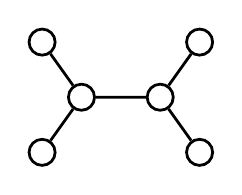
\begin{tikzpicture}[line width = 1pt,
                        solid/.style = {circle, draw, fill = black, minimum size = 0.1cm},
                        empty/.style = {circle, draw, fill = white, minimum size = 0.1cm}]
      \node [empty] (a1) at (0, 0){};
      \node [empty] (a2) at (2, 0){};
      \node [empty] (a3) at (0.5, 0.7){};
      \node [empty] (a4) at (1.5, 0.7){};
      \node [empty] (a5) at (0, 1.4){};
      \node [empty] (a6) at (2, 1.4){};
      \draw (a1) -- (a3) -- (a4) -- (a2);
      \draw (a5) -- (a3);
      \draw (a6) -- (a4);

      \end{tikzpicture} \par
      \normalsize
    \item Let $n$ be the order of the tree, then the size of the tree is $n-1$. The sum of degrees over all vertices is twice the size of the tree, i.e.
        $$ \frac{2}{3} n \times 1 + \frac{1}{3}n \times 3 = 2(n - 1) .$$ \par
        Solve this equation we get $n = 6$. So the only possible tree is: \par
      \small
      \begin{centering}
      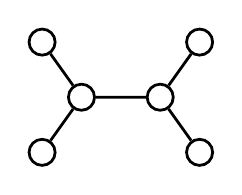
\begin{tikzpicture}[line width = 1pt,
                        solid/.style = {circle, draw, fill = black, minimum size = 0.1cm},
                        empty/.style = {circle, draw, fill = white, minimum size = 0.1cm}]
      \node [empty] (a1) at (0, 0){};
      \node [empty] (a2) at (2, 0){};
      \node [empty] (a3) at (0.5, 0.7){};
      \node [empty] (a4) at (1.5, 0.7){};
      \node [empty] (a5) at (0, 1.4){};
      \node [empty] (a6) at (2, 1.4){};
      \draw (a1) -- (a3) -- (a4) -- (a2);
      \draw (a5) -- (a3);
      \draw (a6) -- (a4);

      \end{tikzpicture} \par
      \end{centering}
      \normalsize
    \end{enumerate}

    \section{[CZ] Problem 4.17}
    \begin{enumerate}
    \item $ $ \\
      \small
      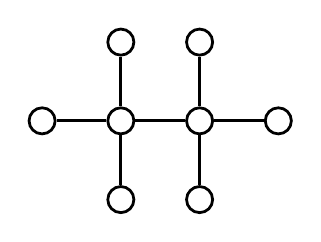
\begin{tikzpicture}[line width = 1pt,
                        solid/.style = {circle, draw, fill = black, minimum size = 0.1cm},
                        empty/.style = {circle, draw, fill = white, minimum size = 0.1cm}]
      \node [empty] (a1) at (1, 0){};
      \node [empty] (a2) at (2, 0){};
      \node [empty] (a3) at (0, 1){};
      \node [empty] (a4) at (1, 1){};
      \node [empty] (a5) at (2, 1){};
      \node [empty] (a6) at (3, 1){};
      \node [empty] (a7) at (1, 2){};
      \node [empty] (a8) at (2, 2){};

      \draw (a1) -- (a4) -- (a7);
      \draw (a2) -- (a5) -- (a8);
      \draw (a3) -- (a4) -- (a5) -- (a6);

      \end{tikzpicture} \par
      \normalsize
    \item Let $n$ be the order of the tree, then the size of the tree is $n-1$. The sum of degrees over all vertices is twice the size of the tree, i.e.
        $$ n \times 75\% \times 1 + n \times 25\% \times 4 = 2(n - 1) .$$ \par
        Solve this equation we get that $n = 8$. The only possible tree is: \par
      \small
      \begin{centering}
      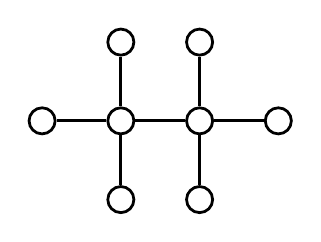
\begin{tikzpicture}[line width = 1pt,
                        solid/.style = {circle, draw, fill = black, minimum size = 0.1cm},
                        empty/.style = {circle, draw, fill = white, minimum size = 0.1cm}]
      \node [empty] (a1) at (1, 0){};
      \node [empty] (a2) at (2, 0){};
      \node [empty] (a3) at (0, 1){};
      \node [empty] (a4) at (1, 1){};
      \node [empty] (a5) at (2, 1){};
      \node [empty] (a6) at (3, 1){};
      \node [empty] (a7) at (1, 2){};
      \node [empty] (a8) at (2, 2){};

      \draw (a1) -- (a4) -- (a7);
      \draw (a2) -- (a5) -- (a8);
      \draw (a3) -- (a4) -- (a5) -- (a6);

      \end{tikzpicture} \par
      \end{centering}
      \normalsize
    \item Let $n$ be the order of the tree, $m > 1$ be the degree of the remaining vertices, then the size of the tree is $n-1$. The sum of degrees over all vertices is twice the size of the tree, i.e.
        $$ n \times 75\% \times 1 + n \times 25\% \times m = 2(n - 1) .$$ \par
        The integer solutions of this equation are: $n = 4, m = 3$ and $n = 8, m = 4$. The corresponding trees are: \par
      \small
      \begin{centering}
      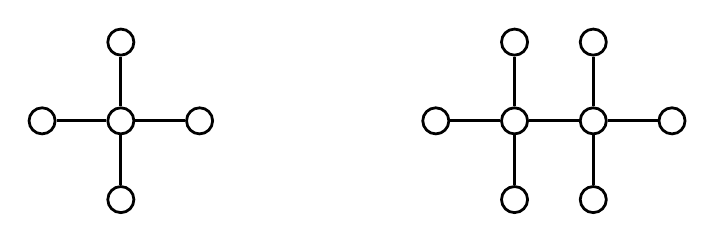
\begin{tikzpicture}[line width = 1pt,
                        solid/.style = {circle, draw, fill = black, minimum size = 0.1cm},
                        empty/.style = {circle, draw, fill = white, minimum size = 0.1cm}]
      \node [empty] (b1) at (-4, 0){};
      \node [empty] (b2) at (-5, 1){};
      \node [empty] (b3) at (-4, 1){};
      \node [empty] (b4) at (-3, 1){};
      \node [empty] (b5) at (-4, 2){};

      \draw (b1) -- (b3) -- (b5);
      \draw (b2) -- (b3) -- (b4);

      \node [empty] (a1) at (1, 0){};
      \node [empty] (a2) at (2, 0){};
      \node [empty] (a3) at (0, 1){};
      \node [empty] (a4) at (1, 1){};
      \node [empty] (a5) at (2, 1){};
      \node [empty] (a6) at (3, 1){};
      \node [empty] (a7) at (1, 2){};
      \node [empty] (a8) at (2, 2){};

      \draw (a1) -- (a4) -- (a7);
      \draw (a2) -- (a5) -- (a8);
      \draw (a3) -- (a4) -- (a5) -- (a6);

      \end{tikzpicture} \par
      \end{centering}
      \normalsize
    \item Let $n$ be the order of the tree, $m > 1$ be the degree of the remaining vertices, then the size of the tree is $n-1$. The sum of degrees over all vertices is twice the size of the tree, i.e.
        $$ n \times 75\% \times 1 + n \times 25\% \times m = 2(n - 1) .$$ \par
        The only integer solution of this equation is $n = 8, m = 2$. The only possible tree is: \par
      \small
      \begin{centering}
      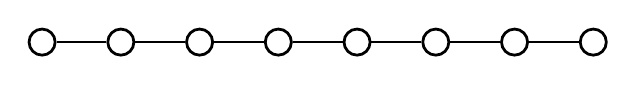
\begin{tikzpicture}[line width = 1pt,
                        solid/.style = {circle, draw, fill = black, minimum size = 0.1cm},
                        empty/.style = {circle, draw, fill = white, minimum size = 0.1cm}]
      \node [empty] (a1) at (0, 0){};
      \node [empty] (a2) at (1, 0){};
      \node [empty] (a3) at (2, 0){};
      \node [empty] (a4) at (3, 0){};
      \node [empty] (a5) at (4, 0){};
      \node [empty] (a6) at (5, 0){};
      \node [empty] (a7) at (6, 0){};
      \node [empty] (a8) at (7, 0){};

      \draw (a1) -- (a2) -- (a3) -- (a4) -- (a5) -- (a6) -- (a7) -- (a8);
      \end{tikzpicture} \par
      \end{centering}
      \normalsize
  \end{enumerate}

  \section{[CZ] Problem 4.18}
  Let $n$ be the order of the tree, $m$ be number of vertices of degree 3, then the size of the tree is $n-1$. The sum of degrees over all vertices is twice the size of the tree, i.e.
        $$ (n-m) \times 1 + m  \times 3= 2(n - 1) $$
  after some algebra we get $m = (n-2)/2$, i.e. $T$ contains $(n-2)/2$ vertices of degree 3.

  \section{[CZ] Problem 4.19}
  \begin{enumerate}
  \item
    Substitute $\sum_i n_i$ for $n$ in $2(n-1) = \sum_i i n _i$, we get $ \sum_i 2n_i - 2 = \sum_i i n _i $, i.e. $ 0 = 2 + \sum_i (i-2) n _i$. Therefore
    $$ n_1 = 2 + n_3 + 2n_4 + 3n_5 + 4n_6 + \cdots $$
  \item Replace $n_i (i>1)$  with the corresponding numbers, we get
    $$ n_1 = 2 + 5 + 2 \times 2 = 11 $$
    i.e. $T$ has 11 end vertices.
  \end{enumerate}
  
  \section{[CZ] Problem 4.19}
  \begin{enumerate}
  \item This statement is false. Here is a counterexample: \par
      \begin{centering}
      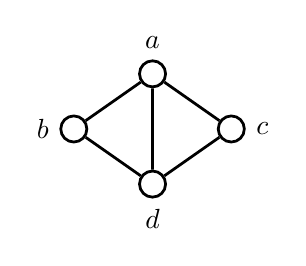
\begin{tikzpicture}[line width = 1pt,
                        solid/.style = {circle, draw, fill = black, minimum size = 0.1cm},
                        empty/.style = {circle, draw, fill = white, minimum size = 0.1cm}]
      \node [empty, label=above:$a$] (a) at (1, 0.7){};
      \node [empty, label=left:$b$] (b) at (0, 0){};
      \node [empty, label=right:$c$] (c) at (2, 0){};
      \node [empty, label=below:$d$] (d) at (1, -0.7){};

      \draw (a) -- (b) -- (d) -- (c) -- (a) -- (d);
      \end{tikzpicture} \par
      \end{centering}
      \normalsize
      In this graph, there are three cycles: $(a,b,d),(a,c,d),(a,b,d,c)$, 4 vertices and 5 edges. Therefore, $m = 5 < n + 2 = 6$.
  \item This statement is true. \par
    Let $n > 0$ be the order of the tree, $r \geq 0$ be the degree of each vertex, then the size of the tree is $n-1$. The sum of degrees over all vertices is twice the size of the tree, i.e.
    $$ nr = 2 (n - 1) .$$
    Integer solutions of this equation are: $n = 1, r = 0$ and $n = 2, r = 1$. Therefore, the only possible trees are: \par
      \begin{centering}
      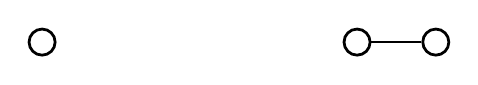
\begin{tikzpicture}[line width = 1pt,
                        solid/.style = {circle, draw, fill = black, minimum size = 0.1cm},
                        empty/.style = {circle, draw, fill = white, minimum size = 0.1cm}]
      \node [empty] (b) at (0, 0){};
      \node [empty] (c) at (1, 0){};
      \node [empty] (a) at (-4, 0){};

      \draw (b) -- (c);
      \end{tikzpicture} \par
      \end{centering}
      \normalsize
  \end{enumerate}
  
  \section{[CZ] Problem 4.21}
  For every vertex $v$ in $\overline{C_{n+2}}$, we have $\deg v = n - 1$, therefore $\delta(\overline{C_{n+2}}) = n - 1$. By Theorem 4.9, $T$ is isomorphic to a subgraph of $\overline{C_{n+2}}$. 
  
  \section{[CZ] Problem 4.22}
  The size of a tree $T$ of order $n$ is $n-1$. The size of $K_n$ has $n(n-1)/2$ . Therefore, the size of $\overline{T}$ is $n(n-1)/2 - (n-1) = (n-2)(n-1)/2$, which is equal to the size of $K_{n-1}$. 
  
  \section{[CZ] Problem 4.23}
  Let $n$ denote the order of $T$, then the size of $T$ is $n-1$, and the size of $\overline{T}$ is $n(n-1)/2 - (n-1) = (n-2)(n-1)/2$. Since $\overline{T}$ is also a tree, the size of $\overline{T}$ is the order of $\overline{T}$ minus 1, i.e.
  $$ (n-2)(n-1)/2 = n - 1. $$
  Solve this equation for $n$, we get $n = 1$ or $n = 4$. For $n = 1$, the tree is trivial. For $n = 4$, the only possible tree whose complement is still a tree is: \par
    \small
    \begin{centering}
      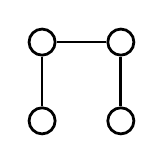
\begin{tikzpicture}[line width = 1pt,
                        solid/.style = {circle, draw, fill = black, minimum size = 0.1cm},
                        empty/.style = {circle, draw, fill = white, minimum size = 0.1cm}]
      \node [empty] (a) at (0, 0){};
      \node [empty] (b) at (1, 0){};
      \node [empty] (c) at (1, 1){};
      \node [empty] (d) at (0, 1){};

      \draw (b) -- (c) -- (d) -- (a);
      \end{tikzpicture} \par
    \end{centering}
    \normalsize
\end{document}
